\chapter{Polar Codes}
\label{ch:polar}

\begin{nontechnical}
\textbf{Polar codes are the newest champions of error correction}---the first codes with mathematical \emph{proof} that they reach Shannon's theoretical limit. That's why 5G uses them!

\textbf{The magic trick:}
\begin{itemize}
\item Take a noisy channel where some bits get through and others don't
\item Apply clever math to ``sort'' the channel into good and bad parts
\item Some sub-channels become PERFECT (polarized to good)
\item Others become USELESS (polarized to bad)
\item Send data on perfect channels, known patterns on bad ones
\item Receiver uses known patterns to decode data!
\end{itemize}

\textbf{Simple analogy:} Imagine 100 students with mixed abilities. Polar coding groups them by strength---put hard problems to strong students, easy problems to weak students. Result: maximum overall success!

\textbf{Real use:} Every 5G phone uses polar codes for control signaling. Huawei championed them, and they're now standardized worldwide.

\textbf{Why they're special:} Only error-correcting codes with mathematical proof of optimality. Turbo and LDPC are great in practice, but polar codes have the theoretical guarantee!
\end{nontechnical}

\section{Overview}

\textbf{Polar codes}, discovered by Erdal Ar{\i}kan in 2008, are the \textbf{first provably capacity-achieving error-correcting codes} with explicit construction. This groundbreaking result earned recognition as one of the most significant advances in coding theory since Shannon's 1948 theorem.

\begin{keyconcept}
Polar codes are \textbf{provably optimal}: they achieve Shannon capacity with explicit construction as block length $N \to \infty$. This theoretical guarantee distinguishes them from empirically-optimized codes like Turbo and LDPC.
\end{keyconcept}

The fundamental principle is \textbf{channel polarization}---recursive channel transformations that split $N$ uses of a binary memoryless channel $W$ into synthetic channels that are either nearly perfect or nearly useless. Information bits are transmitted on the reliable channels, while frozen bits (known values, typically zeros) occupy unreliable positions.

\textbf{Key performance metrics:}
\begin{itemize}
\item Gap to Shannon limit: 0.8--1.5~dB at rate $R = 1/2$, $N = 1024$
\item Decoding complexity: $O(N \log N)$ for successive cancellation (SC)
\item Latency: Low compared to iterative decoders (Turbo/LDPC)
\end{itemize}

\textbf{Standardization:} Polar codes were adopted for \textbf{5G NR control channels} (eMBB and URLLC) in 2016 after competitive evaluation against LDPC and Turbo codes. They excel in short-block, low-latency scenarios critical for control signaling.

\section{Mathematical Description}

\subsection{Channel Polarization}

Channel polarization is the recursive transformation that creates synthetic channels with extreme reliabilities from copies of a base channel.

\subsubsection{Base Transformation (N=2)}

Consider two uses of a binary memoryless channel $W$. The fundamental polar transform combines and splits these into two synthetic channels:
\begin{equation}
\mathbf{y} = \mathbf{u} G_2 = \mathbf{u} \begin{bmatrix} 1 & 0 \\ 1 & 1 \end{bmatrix}
\end{equation}
where:
\begin{itemize}
\item $\mathbf{u} = [u_1, u_2]$ = input bits
\item $\mathbf{y} = [y_1, y_2]$ = combined outputs
\item $G_2$ = base generator matrix
\end{itemize}

This produces:
\begin{equation}
y_1 = u_1 \oplus u_2, \quad y_2 = u_2
\end{equation}

\textbf{Key insight:} After decoding:
\begin{itemize}
\item Channel for $u_1$ is \emph{worse} than $W$ (requires joint decoding)
\item Channel for $u_2$ is \emph{better} than $W$ (uses $u_1$ as side information)
\end{itemize}

This \emph{polarization effect} intensifies with recursion.

\subsubsection{Polarization Theorem}

Ar{\i}kan's fundamental result states that for $N = 2^n$ channel uses:
\begin{equation}
\lim_{n \to \infty} \frac{1}{N} \sum_{i=1}^{N} I(W_i^{(N)}) = I(W)
\end{equation}
where:
\begin{itemize}
\item $I(W_i^{(N)})$ = mutual information of synthetic channel $i$
\item $I(W)$ = capacity of base channel $W$
\end{itemize}

As $N \to \infty$:
\begin{itemize}
\item Fraction $I(W)$ of channels: $I(W_i^{(N)}) \to 1$ (perfect)
\item Fraction $1 - I(W)$ of channels: $I(W_i^{(N)}) \to 0$ (useless)
\end{itemize}

\textbf{Result:} Shannon capacity $C = I(W)$ is achieved by transmitting information only on the nearly-perfect channels.

\subsection{Generator Matrix Construction}

The polar code generator matrix is built via Kronecker products of the base matrix.

\textbf{Base matrix:}
\begin{equation}
G_2 = \begin{bmatrix} 1 & 0 \\ 1 & 1 \end{bmatrix}
\end{equation}

\textbf{General construction:}
\begin{equation}
G_N = G_2^{\otimes n} \quad \text{for } N = 2^n
\end{equation}
where:
\begin{itemize}
\item $G_2^{\otimes n}$ = $n$-fold Kronecker product of $G_2$ with itself
\item $N$ = block length (must be power of 2)
\item $n = \log_2 N$ = recursion depth
\end{itemize}

\textbf{Example for $N=4$:}
\begin{equation}
G_4 = G_2 \otimes G_2 = \begin{bmatrix}
1 & 0 & 0 & 0 \\
1 & 1 & 0 & 0 \\
1 & 0 & 1 & 0 \\
1 & 1 & 1 & 1
\end{bmatrix}
\end{equation}

\textbf{Example for $N=8$:}
\begin{equation}
G_8 = G_2 \otimes G_2 \otimes G_2 = \begin{bmatrix}
1 & 0 & 0 & 0 & 0 & 0 & 0 & 0 \\
1 & 1 & 0 & 0 & 0 & 0 & 0 & 0 \\
1 & 0 & 1 & 0 & 0 & 0 & 0 & 0 \\
\vdots & & & \ddots & & & & \\
1 & 1 & 1 & 1 & 1 & 1 & 1 & 1
\end{bmatrix}
\end{equation}

\subsection{Channel Reliability Metrics}

To select which channels are reliable, we compute reliability metrics for each synthetic channel.

\textbf{Bhattacharyya parameter:}
\begin{equation}
Z(W) = \sum_{y} \sqrt{W(y|0) \cdot W(y|1)}
\end{equation}
where:
\begin{itemize}
\item $W(y|x)$ = transition probability of channel $W$
\item $Z(W) \in [0, 1]$ with lower values indicating higher reliability
\item Perfect channel: $Z = 0$; useless channel: $Z = 1$
\end{itemize}

\textbf{Mutual information:}
\begin{equation}
I(W) = \sum_{y} \sum_{x \in \{0,1\}} W(y|x) \log_2\frac{W(y|x)}{\frac{1}{2}\sum_{x'} W(y|x')}
\end{equation}
where:
\begin{itemize}
\item $I(W) \in [0, 1]$ with higher values indicating higher reliability
\item Perfect channel: $I = 1$; useless channel: $I = 0$
\end{itemize}

\subsection{Density Evolution}

Channel reliabilities can be computed recursively without Monte Carlo simulation.

\textbf{Channel combining (degraded channel):}
\begin{equation}
Z(W^-) \approx 2Z(W) - Z(W)^2
\end{equation}

\textbf{Channel splitting (improved channel):}
\begin{equation}
Z(W^+) \approx Z(W)^2
\end{equation}

\textbf{Starting point for BSC with crossover probability $\epsilon$:}
\begin{equation}
Z_0 = 2\sqrt{\epsilon(1-\epsilon)}
\end{equation}

Apply these recursions $n$ times to obtain reliabilities for all $N = 2^n$ synthetic channels.

\section{Code Construction}

The construction of a polar code involves selecting which bit positions carry information versus frozen (known) bits.

\subsection{Construction Algorithm}

\textbf{Steps for constructing a $(N, K)$ polar code:}

\begin{enumerate}
\item \textbf{Choose block length:} $N = 2^n$ (power of 2)
\item \textbf{Choose code rate:} $R = K/N$ where $K$ = number of information bits
\item \textbf{Compute channel reliabilities:} Use density evolution or Monte Carlo to find $Z(W_i)$ or $I(W_i)$ for $i = 1, \ldots, N$
\item \textbf{Select information set:} $\mathcal{A} = \{$indices of $K$ most reliable channels$\}$
\item \textbf{Select frozen set:} $\mathcal{A}^c = \{$remaining $N-K$ indices$\}$
\end{enumerate}

The resulting code rate is:
\begin{equation}
R = \frac{K}{N}
\end{equation}
where:
\begin{itemize}
\item $R$ = code rate
\item $K$ = number of information bits
\item $N$ = block length
\end{itemize}

\begin{calloutbox}{Frozen Bit Values}
Frozen bits are conventionally set to zero, though any known pattern works. The decoder must know which positions are frozen and their values. This side information is crucial for the successive cancellation algorithm.
\end{calloutbox}

\subsection{Encoding Process}

Given information bits $\mathbf{d} = [d_1, d_2, \ldots, d_K]$ and information set $\mathcal{A}$:

\textbf{Step 1: Form input vector:}
\begin{equation}
u_i = \begin{cases}
d_j & \text{if } i \in \mathcal{A} \text{ (information position)} \\
0 & \text{if } i \in \mathcal{A}^c \text{ (frozen position)}
\end{cases}
\end{equation}

\textbf{Step 2: Encode using generator matrix:}
\begin{equation}
\mathbf{x} = \mathbf{u} G_N
\end{equation}
where:
\begin{itemize}
\item $\mathbf{u} = [u_1, u_2, \ldots, u_N]$ = input vector (information + frozen)
\item $G_N$ = $N \times N$ polar generator matrix
\item $\mathbf{x} = [x_1, x_2, \ldots, x_N]$ = transmitted codeword
\end{itemize}

\textbf{Complexity:} $O(N \log N)$ using FFT-like butterfly structure, avoiding full matrix multiplication.

\subsection{Encoding Example}

Consider $N = 8$, $K = 4$ with information set $\mathcal{A} = \{4, 6, 7, 8\}$ (most reliable channels).

\textbf{Information bits:} $\mathbf{d} = [1, 0, 1, 1]$

\textbf{Input vector} (frozen bits at positions 1, 2, 3, 5):
\begin{equation}
\mathbf{u} = [0, 0, 0, 1, 0, 0, 1, 1]
\end{equation}

\textbf{Encoding:}
\begin{equation}
\mathbf{x} = \mathbf{u} G_8 = [0, 0, 0, 1, 0, 0, 1, 0]
\end{equation}

\textbf{Code rate:} $R = 4/8 = 0.5$

\section{Decoding Algorithms}

\subsection{Successive Cancellation (SC) Decoding}

SC decoding is the foundational algorithm that achieves capacity in the asymptotic limit.

\subsubsection{Algorithm Overview}

The decoder estimates bits sequentially from $u_1$ to $u_N$, using:
\begin{itemize}
\item Received channel outputs $\mathbf{y} = [y_1, \ldots, y_N]$
\item Previously decoded bits $\hat{u}_1^{i-1} = [\hat{u}_1, \ldots, \hat{u}_{i-1}]$
\end{itemize}

For each bit $i$:
\begin{equation}
\hat{u}_i = \begin{cases}
0 & \text{if } i \in \mathcal{A}^c \text{ (frozen bit)} \\
\arg\max_{u_i \in \{0,1\}} P(u_i | \mathbf{y}, \hat{u}_1^{i-1}) & \text{if } i \in \mathcal{A}
\end{cases}
\end{equation}

\subsubsection{Log-Likelihood Ratio (LLR) Recursion}

Efficient implementation uses LLRs defined as:
\begin{equation}
L_i = \log \frac{P(u_i=0 | \mathbf{y}, \hat{u}_1^{i-1})}{P(u_i=1 | \mathbf{y}, \hat{u}_1^{i-1})}
\end{equation}

\textbf{Decision rule:}
\begin{equation}
\hat{u}_i = \begin{cases}
0 & \text{if } L_i \geq 0 \\
1 & \text{if } L_i < 0
\end{cases}
\end{equation}

The LLRs are computed recursively using a butterfly structure in $O(N \log N)$ operations.

\textbf{Left recursion (combining):}
\begin{equation}
L_i^{(s)} = 2 \tanh^{-1}\left(\tanh\left(\frac{L_{2i-1}^{(s+1)}}{2}\right) \cdot \tanh\left(\frac{L_{2i}^{(s+1)}}{2}\right)\right)
\end{equation}

\textbf{Right recursion (splitting):}
\begin{equation}
L_i^{(s)} = L_{2i}^{(s+1)} + (1 - 2\hat{u}_{2i-1}^{(s)}) L_{2i-1}^{(s+1)}
\end{equation}
where:
\begin{itemize}
\item $s$ = stage index ($0$ to $\log_2 N$)
\item $L_i^{(s)}$ = LLR at stage $s$, position $i$
\end{itemize}

\begin{warningbox}
SC decoding is \textbf{sequential}---bit $u_i$ cannot be decoded until $u_1, \ldots, u_{i-1}$ are known. This limits parallelization and can increase latency for large $N$. However, for short blocks ($N \leq 1024$), SC decoding offers lower latency than iterative Turbo/LDPC decoders.
\end{warningbox}

\subsection{SC List (SCL) Decoding}

SCL decoding improves performance by maintaining $L$ candidate paths rather than a single path.

\textbf{Key idea:} At each stage, keep the $L$ most likely decoding paths based on path metrics:
\begin{equation}
PM_i = \sum_{j=1}^{i} \log P(y_j | \hat{u}_1^j)
\end{equation}

\textbf{Typical list sizes:}
\begin{itemize}
\item $L = 1$: Standard SC (baseline performance)
\item $L = 4$: Good performance, moderate complexity
\item $L = 8$ or 16: Near-ML performance, higher complexity
\item $L = 32$: Diminishing returns
\end{itemize}

\textbf{Complexity:} $O(L \cdot N \log N)$

\subsection{CRC-Aided Polar (CA-Polar)}

SCL decoding alone doesn't provide a stopping criterion. CRC-aided polar codes append a cyclic redundancy check to enable path selection.

\textbf{Construction:}
\begin{enumerate}
\item Start with $K_{\text{data}}$ information bits
\item Append $K_{\text{CRC}}$ CRC bits: $K = K_{\text{data}} + K_{\text{CRC}}$
\item Encode using $(N, K)$ polar code
\end{enumerate}

\textbf{Decoding:}
\begin{enumerate}
\item Run SCL decoder with list size $L$
\item Among $L$ paths, select the one passing CRC check
\item If multiple paths pass, select highest path metric
\item If no paths pass, declare error
\end{enumerate}

\begin{keyconcept}
CA-Polar with SCL-8 or SCL-16 achieves near-ML performance, closing the gap between SC decoding and theoretical limits. This combination is standardized in 5G NR.
\end{keyconcept}

Typical CRC lengths:
\begin{itemize}
\item 6 bits: Short blocks ($K < 100$)
\item 11 bits: Medium blocks (5G eMBB control)
\item 16 or 24 bits: Longer blocks, higher reliability
\end{itemize}

\section{Channel Polarization Visualization}

\begin{center}
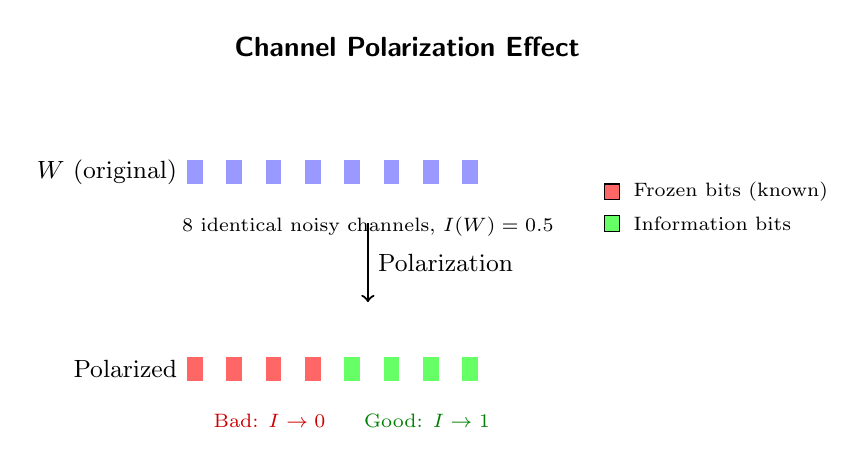
\begin{tikzpicture}[scale=1.0]
% Title
\node[above,font=\sffamily\bfseries] at (3,5.5) {Channel Polarization Effect};

% Original channels
\foreach \i in {1,...,8} {
    \fill[blue!40] (0.5*\i-0.3, 4) rectangle (0.5*\i-0.1, 4.3);
}
\node[left,font=\small] at (0.2, 4.15) {$W$ (original)};
\node[below,font=\scriptsize] at (2.5, 3.7) {8 identical noisy channels, $I(W) = 0.5$};

% Arrow
\draw[->,thick] (2.5,3.5) -- (2.5,2.5) node[midway,right,font=\small] {Polarization};

% Polarized channels
\foreach \i in {1,2,3,4} {
    \fill[red!60] (0.5*\i-0.3, 1.5) rectangle (0.5*\i-0.1, 1.8);
}
\foreach \i in {5,6,7,8} {
    \fill[green!60] (0.5*\i-0.3, 1.5) rectangle (0.5*\i-0.1, 1.8);
}
\node[left,font=\small] at (0.2, 1.65) {Polarized};
\node[below,font=\scriptsize,red!80!black] at (1.25, 1.2) {Bad: $I \to 0$};
\node[below,font=\scriptsize,green!50!black] at (3.25, 1.2) {Good: $I \to 1$};

% Legend
\draw[fill=red!60] (5.5, 3.8) rectangle (5.7, 4.0);
\node[right,font=\scriptsize] at (5.75, 3.9) {Frozen bits (known)};
\draw[fill=green!60] (5.5, 3.4) rectangle (5.7, 3.6);
\node[right,font=\scriptsize] at (5.75, 3.5) {Information bits};

\end{tikzpicture}
\end{center}

\section{Successive Cancellation Decoder Structure}

\begin{center}
\begin{tikzpicture}[
  block/.style={rectangle, draw, minimum width=2.2cm, minimum height=1cm, font=\sffamily\small},
  node distance=2.5cm,
  font=\small
]

% Inputs
\node (input) {\sffamily Received\\$\mathbf{y}$};
\node[block, right of=input] (llr) {LLR\\Computation};
\node[block, right of=llr] (sc) {SC\\Decoder};
\node[right of=sc] (output) {\sffamily Decoded\\$\hat{\mathbf{u}}$};

% Frozen bits feedback
\node[block, below=1.2cm of sc] (frozen) {Frozen Bit\\Memory};
\draw[->,thick] (frozen) -- (sc);

% Arrows
\draw[->,thick] (input) -- (llr);
\draw[->,thick] (llr) -- node[above,font=\scriptsize] {$L_i$} (sc);
\draw[->,thick] (sc) -- (output);

% Description
\node[below=0.3cm of frozen, align=center, font=\scriptsize, text width=5cm] {
Sequential decoding: $\hat{u}_1 \to \hat{u}_2 \to \cdots \to \hat{u}_N$\\
Uses previous decisions $\hat{u}_1^{i-1}$ for bit $u_i$
};

\end{tikzpicture}
\end{center}

\section{Performance Analysis}

\subsection{Capacity-Achieving Property}

Ar{\i}kan proved that polar codes achieve capacity:
\begin{equation}
\lim_{N \to \infty} P_e^{(N)} = 0 \quad \text{for any } R < I(W)
\end{equation}
where:
\begin{itemize}
\item $P_e^{(N)}$ = block error probability for block length $N$
\item $R$ = code rate
\item $I(W)$ = capacity of channel $W$
\end{itemize}

\subsection{Finite-Length Performance}

For practical block lengths, polar codes exhibit characteristic scaling:
\begin{equation}
P_e \approx 2^{-\sqrt{N}}
\end{equation}

This subexponential decay is \emph{slower} than well-designed LDPC/Turbo codes, explaining why polar codes require longer blocks to match their performance.

\subsection{Comparison with Other Codes}

\begin{center}
\begin{tabular}{@{}lcccc@{}}
\toprule
\textbf{Code} & \textbf{Gap to Shannon} & \textbf{Latency} & \textbf{Complexity} & \textbf{Proof?} \\
\midrule
Convolutional & $\sim$6~dB & Low & $O(2^{\nu})$ & No \\
Turbo & 0.5--0.7~dB & High & $O(N \cdot I)$ & No \\
LDPC & 0.3--0.5~dB & Moderate & $O(N \cdot I)$ & No \\
\textbf{Polar (SC)} & 1.5--2.0~dB & Low & $O(N \log N)$ & \textbf{Yes} \\
\textbf{Polar (CA-SCL)} & 0.8--1.2~dB & Low & $O(L N \log N)$ & \textbf{Yes} \\
\bottomrule
\end{tabular}
\end{center}
where:
\begin{itemize}
\item $\nu$ = constraint length (convolutional codes)
\item $I$ = number of iterations (Turbo/LDPC)
\item $L$ = list size (SCL decoding)
\end{itemize}

\textbf{Trade-offs:}
\begin{itemize}
\item \textbf{Polar advantages:} Proven optimality, low latency, systematic construction
\item \textbf{Polar disadvantages:} Sequential decoding, suboptimal at short lengths
\item \textbf{LDPC advantages:} Better short-block performance, parallelizable
\item \textbf{Turbo advantages:} Mature technology, good across all block lengths
\end{itemize}

\section{Worked Example: 5G Control Channel}

Consider a 5G NR control channel transmitting 100 information bits.

\subsection*{System Parameters}

\begin{itemize}
\item Information bits: $K_{\text{data}} = 100$
\item CRC bits: $K_{\text{CRC}} = 11$ (polynomial: CRC-11)
\item Total information: $K = 111$
\item Block length: $N = 256$ (smallest power of 2 $\geq 2K$)
\item Code rate: $R = 111/256 = 0.434$
\item Modulation: QPSK
\item SNR: $E_b/N_0 = 5$~dB
\end{itemize}

\subsection*{Step 1: Code Construction}

Use density evolution for AWGN channel at $E_b/N_0 = 5$~dB to rank channels:
\begin{equation}
\text{Reliability ordering: } W_{128} > W_{192} > W_{224} > \cdots > W_1 > W_2
\end{equation}

Select $\mathcal{A} = \{$111 most reliable indices$\}$ for information + CRC bits.

\subsection*{Step 2: Encoding}

\textbf{Input:}
\begin{itemize}
\item Data: 100 information bits
\item CRC: Compute 11-bit CRC over data
\item Total: $\mathbf{d} = [d_1, \ldots, d_{111}]$
\end{itemize}

\textbf{Form vector $\mathbf{u}$:}
\begin{equation}
u_i = \begin{cases}
d_j & \text{if } i \in \mathcal{A} \\
0 & \text{otherwise (frozen)}
\end{cases}
\end{equation}

\textbf{Encode:}
\begin{equation}
\mathbf{x} = \mathbf{u} G_{256}
\end{equation}

\subsection*{Step 3: Modulation and Transmission}

Map codeword bits to QPSK symbols:
\begin{equation}
s_i = \frac{1}{\sqrt{2}}[(2x_{2i-1} - 1) + j(2x_{2i} - 1)]
\end{equation}

Transmit 128 QPSK symbols over AWGN channel.

\subsection*{Step 4: Decoding}

\textbf{Receiver:}
\begin{enumerate}
\item Demodulate QPSK: compute LLRs for each bit
\item Run CA-SCL decoder with $L = 8$
\item Among 8 candidate paths, select path passing CRC-11 check
\item Extract 100 information bits from decoded vector
\end{enumerate}

\subsection*{Step 5: Performance}

At $E_b/N_0 = 5$~dB:
\begin{itemize}
\item \textbf{Without coding:} BLER $\approx 10^{-1}$ (unacceptable)
\item \textbf{With polar CA-SCL-8:} BLER $\approx 10^{-3}$ (5G target)
\item \textbf{Coding gain:} $\sim$4~dB improvement
\end{itemize}

\begin{calloutbox}[colback=black!8!white,colframe=black]{5G Performance Summary}
\textbf{Result:} Polar codes meet 5G URLLC requirements

For control channels:
\begin{itemize}
\item Low latency: SC/SCL decoding completes in $\sim$10--50~$\mu$s
\item High reliability: BLER $< 10^{-3}$ at practical SNRs
\item Flexible rate matching: Puncturing/shortening for variable payloads
\item Standardized construction: Deterministic, no optimization needed
\end{itemize}

\textbf{Why 5G chose polar:} Perfect fit for short, low-latency control signaling.
\end{calloutbox}

\section{Applications}

\subsection{5G NR Control Channels}

\textbf{Standardized use:}
\begin{itemize}
\item \textbf{eMBB (Enhanced Mobile Broadband):} Downlink/uplink control information (DCI/UCI)
\item \textbf{URLLC (Ultra-Reliable Low Latency):} Mission-critical signaling
\item Block lengths: $N = 32$ to $N = 1024$
\item Code rates: $R = 1/8$ to $R = 7/8$ via rate matching
\end{itemize}

\textbf{5G rationale:}
\begin{itemize}
\item Control channels require low latency ($<$ 1~ms)
\item Short blocks ($K = 20$--200 bits)
\item Variable payload sizes (rate matching flexibility)
\item Proven capacity-achieving property
\end{itemize}

\subsection{Satellite Communications}

Emerging applications in deep-space and satellite links:
\begin{itemize}
\item \textbf{Low SNR regimes:} Near-capacity performance crucial
\item \textbf{Power-limited channels:} Satellite transponders
\item \textbf{Short blocks:} Telemetry and command messages
\end{itemize}

NASA and ESA are evaluating polar codes for future deep-space missions to replace convolutional and Turbo codes.

\subsection{IoT and Machine-Type Communications}

\textbf{Advantages for IoT:}
\begin{itemize}
\item Low-complexity encoding: $O(N \log N)$
\item Short packets: $K = 10$--100 bits
\item Energy efficiency: Simple hardware implementation
\end{itemize}

\textbf{Applications:}
\begin{itemize}
\item Sensor networks
\item Smart meters
\item Industrial automation
\end{itemize}

\subsection{Future Standards}

Polar codes are candidates for:
\begin{itemize}
\item \textbf{6G:} Extension to higher frequencies, extreme reliability
\item \textbf{Quantum communications:} Error correction for quantum channels
\item \textbf{Optical fiber:} High-speed, low-latency FEC
\end{itemize}

\section{Summary}

\begin{center}
\begin{tabular}{@{}ll@{}}
\toprule
\textbf{Parameter} & \textbf{Value} \\
\midrule
Discovery & 2008 (Erdal Ar{\i}kan) \\
Capacity-achieving & Provably optimal ($N \to \infty$) \\
Block length & $N = 2^n$ (power of 2) \\
Code rate & Flexible via construction \\
Encoding complexity & $O(N \log N)$ \\
SC decoding complexity & $O(N \log N)$ \\
SCL decoding complexity & $O(L \cdot N \log N)$ \\
Gap to Shannon (CA-SCL) & 0.8--1.5~dB \\
Latency & Low (non-iterative) \\
Best application & Short blocks, 5G control \\
Standardization & 5G NR (3GPP Release 15) \\
\bottomrule
\end{tabular}
\end{center}

\section{Further Reading}

\begin{itemize}
\item \textbf{Chapter 21:} Turbo Codes---iterative near-capacity codes
\item \textbf{Chapter 22:} LDPC Codes---modern capacity-approaching codes
\item \textbf{Chapter 19:} Convolutional Codes---classical FEC baseline
\item \textbf{Chapter 18:} Forward Error Correction overview
\item \textbf{Chapter 2:} Shannon's Channel Capacity Theorem---theoretical foundation
\item \textbf{Chapter 15:} AWGN Channel---channel model for analysis
\end{itemize}
